Imperative and functional programming models were theorized by the work of Alan Turing, Alonzo Church, Stephen Kleen, Emil Post and many other in the 1930's.
They are different formalizations of the notion of an algorithm, based on automata, symbolic manipulation, recursive function  definitions, and combinatorics.
Those results led Church to conjecture the \emph{Church's thesis}: any intuitively appealing model of computing would be equally powerful as well.

Church's model of computing is called \emph{lambda calculus} and is based on the notion of \emph{parameterized expressions} (parameters are introduced by the letter $\lambda$).
This model allows us to define mathematical functions in a constructive/effective way and is the base inspiration for functional programming.
The computation is done by substituting parameters into expressions, just like we would do in common programming by passing arguments to functions.

\section{Functional programming concepts}
Functional languages like LISP, Scheme, FP, ML, Miranda, Haskell are an attempt to realize Church's lambda calculus.
The key idea is to do everything by composing functions, so we won't have neither mutable state nor side effects.
That said we can see some of the necessary features in this computing model, which not necessarily appear in common imperative languages:
\begin{itemize}
    \item \emph{1st class and high-order functions}: functions can be denoted, passed as arguments and returned, just like they were actual values;

    \item \emph{recursion}: since we have no mutable variables we can't have iterations, so we implement it using recursion;

    \item \emph{powerful list facilities}: recursive functions exploit recursive definition of lists (a list can be seen both as an empty list or as a tuple of value and a list);

    \item \emph{polymorphism}: typically a universal, parametric and implicit version;

    \item \emph{fully general aggregates}: wide use of tuples and records and since variables are immutable data structures can't be modified, they have to be re-created;

    \item \emph{structured function returns}: since there are no side-effects the only way for functions to pass information to the caller is via return values;

    \item \emph{garbage collection}: since it's all static scoping we have unlimited extent for locally allocated data structures and locally defined functions but they can't be allocated on the stack.
\end{itemize}

\subsection{LISP}
LISP (which stands for List Processor) is a family of languages designed in 1958 by John McCarty and implemented in 1960 by Steve Russel.
It has been a main language used to develop AI and presents some features that are not necessary present in other functional languages:
\begin{itemize}
    \item programs, called \emph{S-expressions} are data, in particular lists;
    \item can be self designed so a LISP interpreter can be written in few lines of LISP;
    \item read-evaluate-print interactive loop
\end{itemize}

Some of the variants are:
\begin{itemize}
    \item LISP: which is purely functional, has strong dynamic type checking and is dynamically scoped;
    \item Common Lisp: is the current standard, it's statically scoped and is very rich and complex;
    \item Scheme: statically scoped, has an essential syntax, it's very elegant and is widely used for teaching.
\end{itemize}

\subsection{ML}
Invented by Robin Milner, it's a statically typed, general-purpose programming language.
It's type safe because of it's type inference and formal semantics.
It's compiled but intended for interactive use and it's a combination of Lisp and Algol features like:
\begin{itemize}
    \item it's expression oriented;
    \item it has higher order functions;
    \item it has garbage collection;
    \item it allows to define abstract data types;
    \item it has a module system;
    \item it implements exceptions and exception handling.
\end{itemize}
Although it's impure because it allows side-effects and more over it is a multi-paradigm language.
Some other members of this family of languages are: Standard ML, Caml, OCaml, F\#.

\section{Lambda Calculus}
The syntax of the generic $\lambda$-term is:
$$
    t ::= x | \lambda x.t | t t' | (t)
$$
in which:
\begin{itemize}
    \item $x$: is a generic variable, or name or symbol;
    \item $\lambda x.t$: is the definition of a function which takes $x$ as parameter and computes expression $t$, it's called \emph{abstraction};
    \item $t t'$: is the application of the function $t$ to the argument $t'$.
\end{itemize}
Using this syntax terms can be represented as abstract syntax trees.

Moreover we have the following conventions:
\begin{itemize}
    \item applications associates to left, so:
    $$
        t_1 t_2 t_3 = (t_1 t_2) t_3
    $$

    \item the body of abstraction (function definition) extends as far as possible:
    $$
        \lambda x.\lambda y. x y x = \lambda x. (\lambda y. (x y x))
    $$
\end{itemize}

\subsection{Bound and free variables}
An occurrence of $x$ is free in a term $t$ if it is not in the body of an abstraction $\lambda x.t$, otherwise it is \emph{bound} and the $\lambda x$ is the \emph{binder}.
That means that a variable $x$ is free if there is no function which uses it in the definition of the function, is bounded otherwise.

Terms without free variables are called \emph{combinators}, for example:
\begin{verbatim}
    \lambda x.x
    \lambda x. \lambda y.x
\end{verbatim}
(the first one is the identity function while the second one is the first projection).

\subsection{$\beta$-reduction}
Is the application of the function, so the substitution of the call with the definition (with the correct variable naming).
For example:
\begin{verbatim}
    (\lambda x.x)y = y
\end{verbatim}
we have that the function with parameter $x$ is just $x$ itself, applied on $y$ will return $y$, of course.

\begin{verbatim}
    (\lambda x.x(\lambda x.x))(u r) = u r(\lambda x.x))
\end{verbatim}
in this function we have that variable $x$ is substituted with itself applied to $(\lambda x.x)$, so applying that function over the tuple $u,r$ we have the result.

\begin{verbatim}
    (\lambda x.(\lambda w.x w))(y z) = \lambda w.(y z) w
\end{verbatim}

\subsection{$\lambda$-calculus as a functional language}
We can encode in $\lambda$-calculus most concepts of functional languages.

\subsubsection{Functions with several arguments}
We can specify different arguments in a single expression using $\lambda$-abstractions:
\begin{verbatim}
    \lambda x. \lambda y. <expression>
\end{verbatim}
This is called currying because we are only using functions with a single argument that can return another function, what we've written above can be seen as:
\begin{verbatim}
    f(y)(x)
\end{verbatim}
so basically we call a function $f$ with a parameter $y$, which returns a function which then is called using $x$ as parameter.

Functions that takes parameters and returns functions are called \emph{higher order functions}.

\subsubsection{Boolean operators}
We can encode true and false using lambda expressions:
$$
    T = true ::= \lambda t.\lambda f.t
$$
$$
    F = false ::= \lambda t. \lambda f.f
$$
so to represent true we use a two input function which returns the first argument, to represent false we instead return the second argument.

Using those representations we can build and, or and not representation too:
$$
    and ::= \lambda a. \lambda b. a b F
$$
$$
    or ::= \lambda a. \lambda b . a T b 
$$
$$
    not ::= \lambda a. a F T
$$

\subsubsection{Pair}
We can encode a pair of elements using:
$$
    \lambda f. \lambda s. \lambda b. b f s
$$
to retrieve the first element we just need to apply the pair to the definition of true, and to retrieve the second element we apply the pair to false:
$$
    \xrightarrow{} (pair\,u\,w)\,T
$$
$$
    \xrightarrow{} (\lambda f. \lambda s. \lambda b. b f s) u\, w\, T 
$$
$$
    \xrightarrow{} T\, u\, w 
$$
$$
    \xrightarrow{} u
$$

NB: we can define operators to get first and second using:
$$
    fst ::= \lambda p. p\, T
$$
$$
    snd ::= \lambda p. p\, F
$$

\subsubsection{Church's numerals}
We can define an expression for 0 and a successor function that applied to a number gives us it's successor:
$$
    0 ::= \lambda s. \lambda z.z
$$
$$
    1 ::= \lambda s. \lambda z. s z
$$
$$
    succ = \lambda n. \lambda s. \lambda z\, s\, (n\, s\, z)
$$
so applying \emph{succ} to 2 we get 3:
$$
    succ 2
$$
$$
    \xrightarrow{} (\lambda n. \lambda s. \lambda z. s (n s z)) 2
$$
$$
    \xrightarrow{} \lambda s. \lambda z. s (2 s z)
$$
$$
    \xrightarrow{} \lambda s. \lambda z. s ((\lambda s. \lambda z. s (s z)) s z)
$$
$$
    \xrightarrow{} \lambda s. \lambda z. s ( s (s z)) = 3
$$
basically we build the expression $s^n$ inside the function to represent $n$.

Using the \emph{succ} function we can build arithmetic:
\begin{itemize}
    \item addition:
$$
    plus ::= \lambda m. \lambda n. \lambda s. \lambda z. m\, s\, (n\, s\, z)
$$
    \item multiplication:
$$
    times ::= \lambda m. \lambda n. \lambda s. \lambda z. m\, (n\, s) z
$$
    \item exponentiation:
$$
    pow ::= \lambda m. \lambda n. \lambda s. \lambda z. n\, m\, s\, z
$$
\end{itemize}
and we can build a test to check if an expression evaluates to 0:
$$
    Z ::= \lambda x. x \, F \, not \, F
$$

\subsubsection{Fix-point combinator and recursion}
The following fix-point combinator $Y$, when applied to a function $R$, returns a fix-point of $R$ ($R(YR) = YR$):
$$
    Y = (\lambda y.( \lambda x.y(x\, x) )( \lambda x.y(x\, x) ))
$$
$$
    YR = ( \lambda x.R(x\, x) )( \lambda x.R(x\, x) ) =
$$
$$
    = R(\lambda x.R(x\, x) \, \lambda x.R(x\, x)) = R(YR)
$$
A recursive function definition can be read as a higher-order transformation having a function as first argument, and the desired function is its fix-point:
$$
    R = (\lambda r. \lambda n. Z \, n \, 0 \, (n \, S (r (P \, n))))
$$

Example in haskell:
\begin{verbatim}
    R = \F -> \n -> (n == 0 ? 0 : n + F(n-1))

    (Y R) 3 =
    R (Y R) 3 =
    -- substitute R with it's definition
    -- using (Y R) and 3 as its parameters
    (3 == 0 ? 0 : 3 + (Y R) (3-1)) =
    3 + (Y R) 2 =
    -- keep reducing
    3 + R (Y R) 2 =
    3 + (2 == 0 ? 0 : 2 + (Y R)(2-1)) =
    3 + 2 + (Y R) 1 =
    3 + 2 + R (Y R) 1 =
    3 + 2 + (1 == 0 ? 0 : 1 + (Y R) (1-1)) =
    3 + 2 + 1 + (Y R) 0 =
    3 + 2 + 1 + (0 == 0 ? 0 : 0 + (Y R) (0-1))=
    3 + 2 + 1 + 0 = 6    
\end{verbatim}

\subsubsection{Applicative and normal order evaluation}

\subsection{Order of evaluation}
\begin{itemize}
    \item \emph{applicative order}: arguments are evaluated before applying the function.
    It's also called \emph{eager evaluation} or \emph{parameter passing by value};

    \item \emph{normal order}: functions are evaluated first, arguments are evaluated if and when needed.
    It's sort of \emph{parameter passing by name} and some evaluation can be repeated.
\end{itemize}

The Church-Rosser theorem says that:
\begin{itemize}
    \item if evaluation terminates then the result is unique (result is also called \emph{normal form});
    \item if some evaluation terminates then the normal order evaluation terminates.
\end{itemize}

\subsection{Value and Reference model}
Consider the assignment \verb|a = b|:
\begin{itemize}
    \item \verb|a|: is an \emph{l-value}, which is an expression that must denote a location (an array element, a variable, a dereferenced pointer, etc);

    \item \verb|b|: is an \emph{r-value}, which must be any syntactically valid expression with a type compatible to that of \emph{a}.
\end{itemize}

Around this assignment form we can work in two ways:
\begin{itemize}
    \item value model: languages that adopt this model copy the value of \emph{b} into the location of \emph{a};
    \item reference model: languages that adopt this model copy a reference to the value of \emph{a} resulting in shared data values via multiple references (also called \emph{call by sharing}).
\end{itemize}

Lisp, Scheme, ML, Haskell, Smalltalk adopt the reference model while Java uses the value model for built-in types and reference for objects, just like C\# and others.
We will define:
\begin{itemize}
    \item reference to \emph{X} as the address of the cell where \emph{X} is stored;
    \item pointer to \emph{X} as the location containing the address of \emph{X}.
\end{itemize}
we can use the value model based to emulate reference model using pointers.

\subsubsection{Parameter passing in Algol 60}
Algol 60 uses \emph{call by name} by default, but also call by value.
Effect of call by name is that the actual parameter is coped wherever the formal parameter appears in the body, then the result code is executed.
The actual parameter is evaluated a number of times that depends on the logic of the program.
Since the actual parameter can contain names, it is passed in a closure with the environment at invocation time (called a thunk).
Call by name is powerful but makes programs difficult to read and to debug, so it has been dismissed in subsequent versions of algol.

\subsubsection{Summary of parameter passing modes}
\begin{figure}[H]
    \centering
    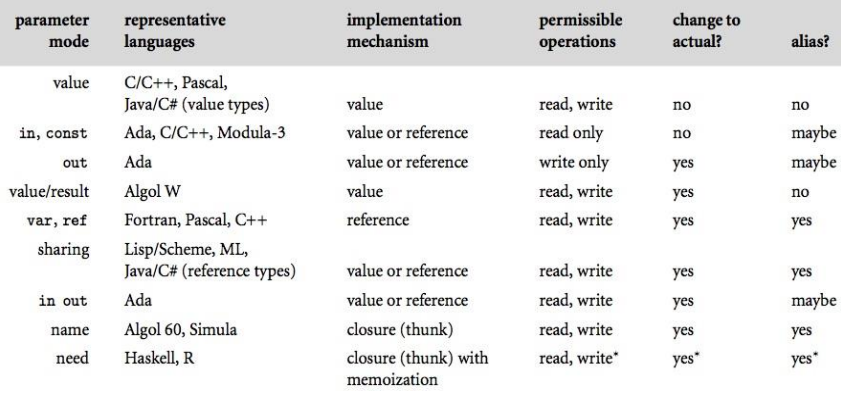
\includegraphics[width=300px]{images/7_Functional_Programming/parameter_passing_summary.png}
\end{figure}


\section{Haskell}
It's designed by a committee in 80's-90's and is though to unify efforts in lazy languages.
It has several features in common with ML but some of them differs:
\begin{itemize}
    \item it has type inference, implicit parameter polymorphism and ad-hoc polymorphism via overloading;
    \item it's lazily evaluated and implements tail recursion and continuations;
    \item it's purely functional and it has precise management of effects.
\end{itemize}

\subsection{Overview of Haskell}
Haskell has a REPL called \verb|ghci| which infers type before compiling or executing.
The type system does not allow casts or similar things.

\subsubsection{Overview by type}
Among the types available in the language we have:
\begin{itemize}
    \item booleans with constants \verb|True|, \verb|False|.
    And some operators to work with like: \verb|not|, \verb|and|, \verb|or|, \verb|if ... then ... else ...|

    \item characters and strings: characters are surrounded with \verb|'| and strings are lists of chars.

    \item numbers: 
    \item tuples: is the basic compound type, it allows to structure different type of data on a single structure:
\begin{verbatim}
    ("AP", 2017)
    -- this tuple is a pair and we can use the follownig selectors
    -- fst: to access the first element
    -- snd: to access the second element
    -- usage: fst (..)

    (1, True, "AP")
    -- tuple of three arguments
\end{verbatim}

    \item lists: normal array of values, it must contains all elements of the same type
\begin{verbatim}
    []
    -- empty list
    -- some operator for the lists are:
    -- 1 : [..] : to add an element to the top of the list
    -- [1,2] ++ [3,4] : to concatenate two lists
    -- head: to get first element of the list
    -- tail: to get rest of the list
    -- reverse: used to reverse the order of the elements in the list
\end{verbatim}

    \item records: it's kind of a named tuples, like C structs:
\begin{verbatim}
    data Person = Person {
        firstName :: String,
        lastName :: String
    }
    -- we define the data type

    hg = Person {
        firstName = "Giovanni",
        lastName = "Boccaccio"
    }
    -- we allocate a record
\end{verbatim}
\end{itemize}

\subsubsection{List constructors}
There exists different ways to build a list:
\begin{itemize}
    \item simple range:
\begin{verbatim}
    [first..second]
\end{verbatim}
    will build a list with all the elements from first to second using 1 as increment.

    \item range with step:
\begin{verbatim}
    [first,second..last]
\end{verbatim}
    will build a list with all the elements from first to last using \verb|second-first| as step.

    \item unconstrained range:
\begin{verbatim}
    [first..]
\end{verbatim}
    infinite list starting from first.

    \item unconstrained range with step:
\begin{verbatim}
    [first,second..]
\end{verbatim}
\end{itemize}
of course this structure works with characters too and if the elements are in reverse order we will get descending lists.

We can use some operators on the range we've specified:
\begin{itemize}
    \item \verb|take|: it's used to crop the range after $n$ elements:
\begin{verbatim}
    take 10 [1..]
\end{verbatim}
    will take first 10 elements of the infinite list built.

    \item \verb|cycle|: used on a list repeats the list infinitely times:
\begin{verbatim}
    take 10 (cycle [1,2])
    -- [1,2,1,2,1,2,1,2,1,2]
\end{verbatim}

    \item \verb|repeat|: used on element to repeat it infinitely times:
\begin{verbatim}
    take 10 (repeat 5)
    -- [5,5,5,5,5,5,5,5,5,5]
\end{verbatim}
\end{itemize}

\subsubsection{Binding variables}
Variables are bound to expressions without evaluating them until it is strictly necessary.
That's called lazy evaluation.
The scope of this binding is the rest of the session (all the program).
The keyword to define a new binding is \verb|let| but it's optional to use.
\begin{verbatim}
    let a = 6
    b = a + 2
    -- let keyword is optional
    -- moreover the calculation is not done
    -- because of lazyness of the language

    b
    -- now the calculation is actually done
\end{verbatim}

\subsubsection{Patterns and declarations}
Patterns can be used in place of variables in order to build variables by destructuring data types:
\begin{verbatim}
    tuple = ("Foo", "Bar")
    (x,y) = tuple
    -- the tuple is destructured and
    -- x gets assigned "Foo"
    -- while y gets assigned "Bar"

    list = [1,2,3,4]
    z:zs = list
    -- list gestr destructured and
    -- z gets assignes 1 (head)
    -- while zs gets assigned [2,3,4] (tail)
\end{verbatim}

\subsubsection{Anonymous functions}
We can declare operators (functions) without name and assign them to variables to be used later or to be used during the creation:
\begin{verbatim}
    (\x -> x+1)
    -- creates an anonymous function but
    -- then it gets dropped

    (\x -> x+1) 5
    -- create an anonymous function and then
    -- applies it to the value 5
    
    f = \x -> x+1
    -- creates an anonymous function and then
    -- it gets binded to the variable f

    f 7
    -- calls function f on value 7
\end{verbatim}

Of course functions can be defined using patterns in order to get structures as input:
\begin{verbatim}
    h = \(x,y) -> x+y
    -- takes a pair as input

    h (3,4)
    -- correct invocation
    h 3 4 
    -- wrong invocation because it needs a pair

    k = \(z:zs) -> length zs
    -- takes a list as input, splitted in it's
    -- head and tail representation

    k "hello"
    -- correct invocation
\end{verbatim}

\subsubsection{Function declarations}
Of course function can be declared as well using the following notation:
\begin{verbatim}
    <name> <pattern> = <expression>
\end{verbatim}
and we can create different implementations for the different patterns:
\begin{verbatim}
    length [] = 0
    -- version for empty list
    length (x:s) = 1+ length(s)
    -- version for non empty list which uses recursion
\end{verbatim}


\subsection{Laziness}
Haskell is a lazy language, which means that functions and data constructors don't get evaluated until they are needed. 
In several languages there is this concept inside the if-then-else construct or inside the short circuit of and and or logical operators.

In Haskell instead this mechanism is built on top of \emph{normal order evaluation} and \emph{call by need} parameter passing so an expression passed as argument is bound to the formal parameter, but it is evaluated only if its value is needed.

Moreover the argument is evaluated only the first time, then using the \emph{memoization} the result is saved and further uses of the argument do not need to re-evaluate it.

This parameter passing combined with \emph{lazy data constructors} allows to construct potentially infinite data structure and recursive infinitely without necessarily causing non-termination.

NB: lazy evaluation works fine with purely functional languages because computation doesn't allows side effects, though sometimes it's necessary to deal with side effects so Haskell implements concepts of monads.

\subsubsection{Parameter passing mechanisms}
There exists three ways to pass parameters:
\begin{itemize}
    \item in;
    \item in/out;
    \item out.
\end{itemize}

The mechanisms for parameter passing are:
\begin{itemize}
    \item call by value: using in;
    \item call by reference: using in+out;
    \item call by result: using out;
    \item call by value/result: using in+out;
    \item call by need: using in;
    \item call by sharing: using in/out;
    \item call by name: using in+out.
\end{itemize}
the last three are the one used in Haskell.

\subsection{List comprehension}
List comprehension is a notation for constructing new lists from old ones:
\begin{verbatim}
    myData = [1..10]
    twiceData = [2*x | x <- myData]
    -- it literally says to collect 2*x for each x in myData

    twiceFilteredData = [2*x | x <-myData, x `mod` 2 == 0]
    -- it says to collect 2*x for each x in myData that has mod 2 equals to 0
\end{verbatim}
it is similar to the set definition in math:
$$
\{ x | x \in A \land x > 6 \}
$$
Of course more predicates can be specified, and more starting lists can be used to compute more complex results.


\subsection{Datatype and pattern matching}
In haskell we can declare new data type with the following syntax:
\begin{verbatim}
    data <name> ::= <clause> | ... | <clause>
    <clause>    ::= <constructor> | <constructor> <type>
\end{verbatim}
some examples:
\begin{verbatim}
    data Color =  Red | Yellow | Blue
    -- create Color data type which has
    -- only Red, Yellow and Blue as values

    data Atom = Atom String | Number Int
    -- elements can be Atom with every string
    -- and Number with every number

    data List = Nil | Cons (Atom, List)
    -- we define a list as Nil or a tuple
    -- of an Atom and another List
    -- it's a recursive definition of a list
\end{verbatim}
type name and constructors must be capitalized.

So we can use those data type definitions to build recursive data structures:
\begin{verbatim}
    data Tree = Leaf Int | Node (Int, Tree, Tree)
\end{verbatim}
we are saying that a tree can be a Leaf which holds an integer number or can be a Node which holds an int and two more trees.

We can use the constructor we've defined inside pattern matching in function definition, this means that we define an overloaded function which has different implementation based on the pattern we've encountered.
For example let's compute the sum of a given tree:
\begin{verbatim}
    sum (Leaf n) = n
    sum (Node(n, t1, t2)) = n + sum(t1) + sum(t2)
\end{verbatim}

Moreover another use case for the pattern matching is inside the case expression, we can evaluate a variable and based on it's type we can perform different actions:
\begin{verbatim}
    data Exp = Var Int | Const Int | Plus (Exp, Exp)

    case e of
        Var n -> ...
        Const n -> ...
        Plus(e1, e2) -> ...
\end{verbatim}
in the case statement indentation matters!

\subsubsection{Function types}
In Haskell the notation \verb|f :: A -> B| means that the function can be applied to every element in the set \verb|A|, in which set means a type, while the result can be in the set \verb|B| or the function can never terminate.

Moreover if \verb|f| is a standard binary function then \verb|`f`| is the infix version, so the operator is between it's parameter:
\begin{verbatim}
    1 + 2
    -- + is an infix operator because
    -- it's placed between it's operands
\end{verbatim}
while if \verb|x| is an infix binary operator then \verb|(x)| is its prefix version.
\begin{verbatim}
    (+) 1 2
    -- here we are using the prefix notation
    -- of the operator +
\end{verbatim}

\subsection{Recursion}
In functional programming loops are replaced by recursion:
\begin{verbatim}
    length' [] = 0
    length' (x:s) = 1 + length' (s)
\end{verbatim}
we've defined the \verb|length'| function to evaluate the length of a list using a recursive definition with guards and pattern matching.

\begin{verbatim}
    take' n _
        | n <= 0 = []

    take' _ [] = []
    take' n (x:xs) = x : take' (n-1) xs
\end{verbatim}
in this multiple definition we are saying:
\begin{itemize}
    \item if the function is called with a number, any list but the number is $<=$ 0, then the result is an empty list;
    \item if the function is called with any number but an empty list, then the result is an empty list;
    \item if the function is called with any number and any list, then return the concatenation of the first element in the list and the result of \verb|take'| called on $n-1$ and the tail of the list.
\end{itemize}

\subsection{Higher order functions}
Functions that take other functions as arguments or return a functions as a result are higher order functions and are one of the main concepts of functional programming.
\begin{verbatim}
    applyTo5 f = f 5
    -- this function is of type
    -- (t1 -> t2) -> t2
    -- so it take a function from
    -- type t1 to type t2 and
    -- returns a value of type t2

    applyTo5 succ
    -- will return 6
    applyTo5 (7 +)
    -- will return 12
\end{verbatim}

Those functions can be used on alternative syntax, for example the stream-like one:
let's define an operator which takes an input value and a function and applies that function to that value:
\begin{verbatim}
    (|>) :: t1 -> (t1 -> t2) -> t2
    (|>) a f = f a
\end{verbatim}
now we can chain calls to this function in order to build a stream-like computation:
\begin{verbatim}
    length(tail (reverse [1,2,3]))
    -- return 2
    -- can be rewritten as:

    [1,2,3] |> reverse |> tail |> length
\end{verbatim}

Any curried function with more than one argument is an higher-order function because it's a function which is applied to one argument and return a function that needs to be evaluated to the next argument and so on and so forth.

\subsubsection{map combinator}
map is a function that given a function and a collection applies that function to any element of the collection, then returns a new collection made of the obtained values:
\begin{verbatim}
    map :: (a->b) -> [a] -> [b]
    -- it takes a function from type a to type b
    -- then takes a collection of elements of type a
    -- and return a collection of elements of type b

    map _ [] = []
    map f (x:xs) = f x : map f xs
\end{verbatim}
some examples:
\begin{verbatim}
    map (+3) [1, 5, 3, 1, 6]
    -- returns [4, 8, 6, 4, 9]
\end{verbatim}

\subsubsection{filter combinator}
filter is a function that takes a collection and a boolean predicate and returns the collection of the elements that satisfies the predicate:
\begin{verbatim}
    filter :: (a -> Bool) -> [a] -> [a]
    -- it takes a function from type a to Boolean
    -- then takes a collection of elements of type a
    -- and return a collection of elements of type a

    filter _ [] = []
    filter p (x:xs)
        | p x = x : filter p xs
        | otherwise = filter p xs
\end{verbatim}
some examples:
\begin{verbatim}
    filter (>3) [1,5,3,2,1,6,4,3,2,1]
    -- returns [5,6,4]
\end{verbatim}

\subsubsection{reduce combinator}
reduce takes a collection, an initial value and a function (binary function), and combines the elements in the collection according to the provided function.
There exists several variants:
\begin{itemize}
    \item \verb|foldr|: folds values from end to beginning of list;
    \item \verb|foldl|: folds values from beginning to end of list;
    \item \verb|foldr1|, \verb|foldl1|: variants for non empty lists.
\end{itemize}
\begin{verbatim}
    foldr :: Foldable t => (a -> b -> b) -> b -> t a -> b
    foldr f z [] = z
    foldr f z (x:xs) = f x (foldr f z xs)
    -- return value if empty list
    -- return the application of f to first element
    -- of list and the result of fold to the rest of the list

    foldl :: Foldable t => (b -> a -> b) -> b -> t a -> b
    foldl f z [] = z
    foldl f z (x:xs) = foldl f (f z x) xs      
\end{verbatim}

\subsection{Examples of functional approach over imperative}
Let's write code to identify if a string \verb|x| is a substring of a string \verb|s|.
We can say that \verb|x| is substring of \verb|s| if among all the suffices of \verb|s| there is at least one who has as prefix the string \verb|x|.
To get all the suffixes we can use:
\begin{verbatim}
    suffixes :: [a] -> [[a]]
    suffixes [] = [[]]
    suffixes (x:xs) = (x:xs) : suffixes xs
    -- suffixes of empty string is an empty set
    -- suffixes of a string is the concatenation of
    -- the string itself and the suffixes of the tail
    -- of the string
\end{verbatim}

To check if a string is suffix of another one we can use:
\begin{verbatim}
    isPrefixOf :: a => [a] -> [a] -> Bool
    isPrefixOf [] x = True
    isPrefixOf (y:ys) [] = False
    isPrefixOf (y:ys) (x:xs) = 
        if (x==y) then isPrefixOf ys xs else False
\end{verbatim}

Then we can use a function to check if in a list there is at least one True:
\begin{verbatim}
    or :: [Bool] -> Bool
    or [] = False
    or (x:xs) = x || or xs
\end{verbatim}

In the end we fit everything together:
\begin{verbatim}
    isSubString :: [a] -> [a] -> Bool
    x `isSubString` s = or [x `isPrefixOf` t | t <- suffixes s]
\end{verbatim}

\subsection{Notes}
Iteration and recursion are equally powerful but a procedure call is much more expensive than a jump, so iterative implementation are, in general, better from a performance point of view, although recursion sometimes is much more expressive as for example in a tree traversal or some mathematical definitions.
The use of combinators like map, reduce, and so on can be seen and optimized by compilers, so lately there is not so much gap between the two versions.

\subsubsection{Tail recursion}
Tail-recursive functions are functions in which no operations follow the recursive calls in the function, so the function returns immediately after the recursive call.
As an example:
\begin{verbatim}
    int tail_recursive_fun(...){
        ...
        return tail_recursive_fun(...);
    }

    int not_tail_recursive_fun(...){
        ...
        return 1 + not_tail_recursive_fun(...);
    }
\end{verbatim}
Tail recursive implementations can reuse the subroutine's frame on the run-time stack avoiding the creation of a new one, this translates into a performance improvement.
So the compiler can try to improve everything translating recursion to tail recursion and translating the recursive calls to jumps to the beginning of the function.

To convert a recursive call to a tail-recursive call we ca try to remove the work after the recursive call and include it in some other form as a computation that then is passed as parameter to the recursive call:
\begin{verbatim}
    -- recursive fibonacci
    fib = \n -> if n == 0 then 1
                else if n == 1 then 1
                else fib(n-1) + fib(n-2)

    -- tail recursive fibonacci
    fibhelper = \f1 f2 i ->
                if (i==1) then f2
                else fibhelper f2, (f1+f2), (i-1)

    fib = \n -> fibhelper 0 1 n
\end{verbatim}

\subsection{Polymorphism}
Haskell has both type inference and overloading as polymorphism type.
In particular the overloading is complex because it is not always easy to understand to which type of data a function can be applied:
\begin{itemize}
    \item \verb|length :: [w] -> Int|: is fully polymorphic because the length of a list is defined despite the type of the list;
    \item \verb|member :: [w] -> w -> Bool|: membership only works for types that support equality;
    \item \verb|sort :: [w] -> [w]|: sorting can only be done on types that support ordering.
\end{itemize}
A possible implementation for this feature could be to define multiple functions for the different type, but this approach is not widely used because of exponential growth in number of versions.

NB: in ML the basic operators such as + and * can be overloaded but not the functions defined from them, but this approach is not so good because programmers cannot define functions that implementation might support as well.

The solution adopted by Haskell is a generalization of the \emph{eqtype} from ML:
\begin{itemize}
    \item it provides coincise types to describe overloaded functions;
    \item allows users to define functions using overloaded operations;
    \item allows users to declare new collections of overloaded functions;
    \item fits within type inference framework.
\end{itemize}
Let's think of a \verb|sort| function with a comparison operator as an argument, now the function is parametric and can be used for every type that implements a comparison function.

We can generalize the idea: we build functions that take as parameter a \emph{dictionary} that provides implementation for the overloaded operators, then inside the function we will call the correct implementation for that operator from that dictionary.
This mechanism is already done by the language when using the \emph{type class} without the need to do it by ourselves.

\subsection{Type Class}
To declare a new type class we need to define a set of operations and give to this set a name.
For example the type class \verb|Eq a| defines both the operations \verb|==| and \verb|\=| both with type \verb|a -> a -> Bool|.
Then to add a specific type to the type class we need to add the implementations of that operations for the specified type.

Now we can use the \emph{type constraints} (or qualified types) in order to express the operations required for a type in the function declaration.
For example if we want that the \verb|member| function can only be used for type that admit an equality operator we will use:
\begin{verbatim}
    member :: Eq w => w -> [w] -> Bool
    -- can be readed as: for all the types w
    -- that support the Eq operations
\end{verbatim}

\subsubsection{Definition}
To define a new type class the syntax is:
\begin{verbatim}
    class Num a where
      (+)     :: a -> a -> a
      (*)     :: a -> a -> a
      negate  :: a -> a
      ...
\end{verbatim}
so the class definition only declares the signature for the functions that a type must implement in order to follow that type class.

To define, instead, the function themselves for the specified type the syntax is:
\begin{verbatim}
    instance Num Int where
        a + b     = intPlus a b
        a * b     = intTimes a b
        negate a  = intNeg a
        ...
\end{verbatim}

NB: \verb|intPlus|, \verb|intTimes|, \verb|intNeg| are builtin primitives.

\subsubsection{Compilation}
Writing:
\begin{verbatim}
    square :: Num n => n -> n
    square x = x*x
\end{verbatim}
leads the compiler to generate something like:
\begin{verbatim}
    square :: Num n -> n -> n
    square d x = (*) d x x
\end{verbatim}
so the constraint \verb|Num n =>| becomes a new parameter to the function, the dictionary of the specified type.

Moreover the class declaration:
\begin{verbatim}
    class Num n where
      (+)    :: n -> n -> n
      (*)    :: n -> n -> n
      negate :: n -> n
\end{verbatim}
is translated into:
\begin{verbatim}
    data Num n
      = MkNum (n -> n -> n)
            (n -> n -> n)
            (n -> n)
            ...

    (*) :: Num n -> n -> n -> n
    (*) (MkNum _ m _ ...) = m
\end{verbatim}
basically a dictionary of the \verb|Num| operations for type n and a set of selector functions.

In the end when declaring an instance:
\begin{verbatim}
    instance Num Int where
      a + b     = intPlus a b
      a * b     = intTimes a b
      negate a  = intNeg a
      ...
\end{verbatim}
the compiler produces:
\begin{verbatim}
    dNumInt :: Num Int
    dNumInt = MkNum intPlus
                    intTimes
                    intNeg
                    ...
\end{verbatim}
which is a value declaration for a dictionary.

Of course in case of multiple type classes used inside a function declaration there will be more dictionaries passed as parameters.

\subsubsection{Compositionality}
This approach solves the problem of functions using overloaded operators because we just need to detect overloaded operators and then add the dictionary to the function signature.

Moreover we can build compound instances from simpler ones, so for example we can build an \verb|Eq [a]| type with the constraint \verb|Eq a|:
\begin{verbatim}
    class Eq a => Eq [a] where
      (==) [] [] = True
      (==) (x:xs) (y:ys) = x==y && xs == ys
      (==) _ _ = False
\end{verbatim}


\subsubsection{Some type classes}
Some of the type classes already built-ins:
\begin{itemize}
    \item Eq: equality;
    \item Ord: comparison;
    \item Num: numerical operations;
    \item Show: convert to string;
    \item Read: convert from string;
    \item generic programming, reflections, monads, ...
\end{itemize}

\subsubsection{Subclasses}
We can declare types classes as subclasses of another class, which means that basically it extends the type whose it's subclass:
\begin{verbatim}
    class Eq a => Num a where
        ...
\end{verbatim}
we are saying that \verb|Num| is subclass of \verb|Eq|.
\begin{figure}[H]
    \centering
    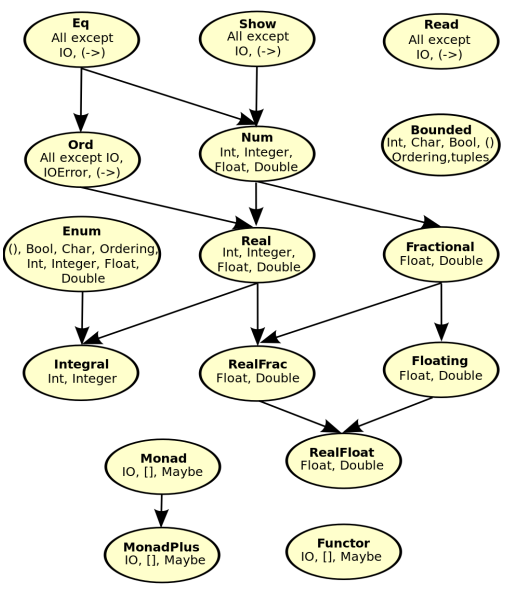
\includegraphics[width=200px]{images/7_Functional_Programming/type_classes_hierarchy.png}
    \caption{Type Classes hierarchy}
\end{figure}

\subsubsection{Default methods}
A type class can also define default methods (of course it can be overridden by a more specific implementation):
\begin{verbatim}
    class Eq a where
    (==) :: a -> a -> Bool
    x == y = not (x /= y)

    (/=) :: a -> a -> Bool
    x /= y = not (x==y)
\end{verbatim}

\subsubsection{Deriving}
For the type classes \verb|Read|, \verb|Show|, \verb|Bounded|, \verb|Enum|, \verb|Eq|, \verb|Ord| the compiler can generate instance declarations automatically.
For example \verb|Show| is a lot useful when defining custom types and we want to have a default print implementation.
\begin{verbatim}
    data Color = Red | Green | Blue
        deriving (Show, Read, Eq, Ord)
\end{verbatim}

\subsubsection{Numeric literals}
Literals are overloaded, so are functions that call the \verb|fromInteger| implementation of the \verb|Num| type class.

\subsection{Type inference}
Type checking means that the compiler examines the body of each function and uses declared types to check for consistency.
In type inference instead the compiler examines the code, which has no type information, and infers the most general types that could have been declared.

NB: ML and Haskell are designed to make type inference feasible because it's not always possible. 

The type inference by itself reduces syntactic overhead of expressive types, still allowing for static type checking, moreover it is guaranteed to produce the most general types.
It has originally been developed for functional languages but now is widely used in any kind of languages.
In the end it is an illustrative example of a flow-insensitive static analysis algorithm.

\subsubsection{History}
It has originally been invented by Haskell Curry and Robert Feys for the simply typed lambda calculus, then it has been extended to a richer language and proved it always produced the most general type by J. Roger Hindley.

Then Robin Milner developed an equivalent algorithm called algorithm W.
In 1982 Luis Damas proved the algorithm was complete.
In the end in 1989 Kanellakis, Mairson and Mitchell proved that the problem was exponential-time complete but usually it is linear in practice (exponential in the depth of polymorphic declarations).

\subsubsection{Basic idea}
We'll use uHaskell, which is a subset of Haskell, to understand type inference.
Let's take for example the following declaration:
\begin{verbatim}
    f x = 2 + x
\end{verbatim}
the algorithm will evaluate the syntax and will find the following hypothesis:
\begin{itemize}
    \item \verb|+| has type \verb|Int -> Int -> Int|;
    \item \verb|2| has type \verb|Int|
\end{itemize}
so under those constraints we need that \verb|x| has type \verb|Int| too, so in the end the function \verb|f| has type \verb|Int -> Int|.

Less generically the algorithm:
\begin{itemize}
    \item parses the program text in order to construct a parse tree:
    \begin{figure}[H]
        \centering
        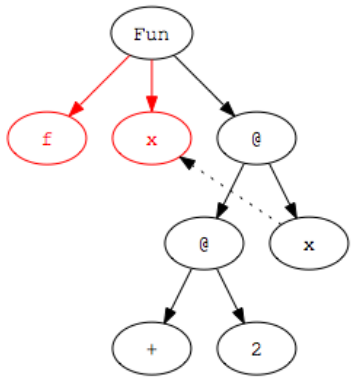
\includegraphics[width=200px]{images/7_Functional_Programming/type_inference_algorithm_1.png}
        \caption{Parse tree}
    \end{figure}
    the binary node \verb|@| represent a function application, while the ternary node \verb|Fun| represent a function definition.
    Moreover infix operators are converted to curried function application: \verb|2 + x| becomes \verb|(+) 2 x|;

    \item assigns type variables to nodes:
    \begin{figure}[H]
        \centering
        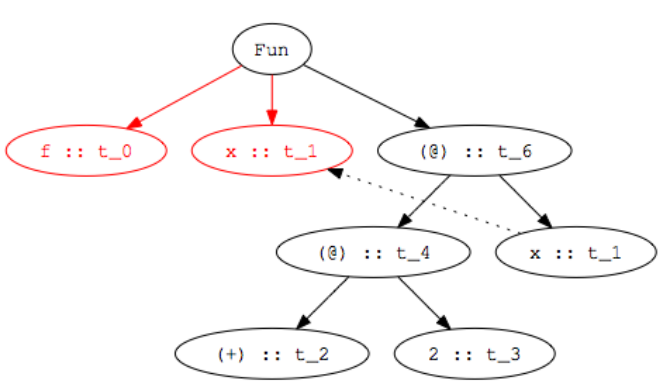
\includegraphics[width=300px]{images/7_Functional_Programming/type_inference_algorithm_2.png}
        \caption{Variables assigned to node}
    \end{figure}
    Of course different occurrences of the same variable will have the same type.

    \item build constraints:
    traversing the tree we build the constraints:
    \begin{itemize}
        \item the literals themselves have some type so we can add them as constraints;

        \item the built-ins operators and the known functions have already known types;

        \item at the function application we have that the type of \verb|f| must be from a domain to a range, the domain of the function must be the type of the argument and the range of the function must be result of the application itself, so we can build a constraint (according to the picture we'll have: \verb|t_0=t_1->t_2|);

        \item at the function declaration we have that the type of the function must go from the domain to the range, so we have the same constraint of the function application;
    \end{itemize}

    \item solve constraint using \emph{unification}: once we've written all the constraints we can solve them by substitution:
    \begin{verbatim}
        t_0 = t_1 -> t_6
        t_4 = t_1 -> t_6
        t_2 = t_3 -> t_4
        t_2 = Int -> Int -> Int
        t_3 = Int
    \end{verbatim}
    so for example from the constraints of \verb|t_2| we can build:
    \begin{verbatim}
        t_2 = t_3 -> t_4 => Int -> (Int -> Int) = t_2
        --> t_3 = Int
        --> t_4 = Int -> Int
    \end{verbatim}
    then we join the constraints for \verb|t_4| obtaining:
    \begin{verbatim}
        t_4 = t_1 -> t_6 => Int -> Int
        --> t_1 = Int
        --> t_6 = Int
        --> t_0 = Int -> Int
    \end{verbatim}

    \item determine type of declaration.    
\end{itemize}

\subsubsection{Inferring polymorphic types}
In case of polymorphic types during the constraint solve we'll have unconstrained type variables, those variables will become polymorphic types.

\subsubsection{Polymorphic datatypes}
Functions may have multiple clauses:
\begin{verbatim}
    length [] = 0
    length (x:rest) = 1 + (length rest)
\end{verbatim}
in those cases we infer separate type for each clause, then we combine them by adding constraint that all clauses must have the same type.
In case of recursive calls the function has the same type as its definition:
\begin{figure}[H]
    \centering
    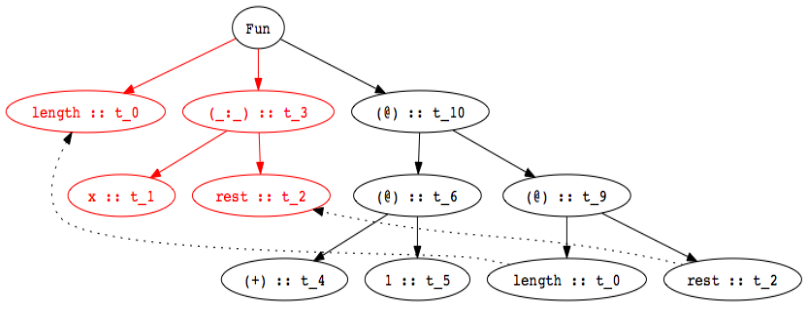
\includegraphics[width=350px]{images/7_Functional_Programming/type_inference_recursive.png}
    \caption{Parse tree of recursive call}
\end{figure}
we'll have those constraints:
\begin{verbatim}
    t_0 = t_3 -> t_10
    t_3 = t_2
    t_3 = [t_1]
    t_6 = t_9 -> t_10
    t_4 = t_5 -> t_6
    t_4 = Int -> Int -> Int
    t_5 = Int
    t_0 = t_2 -> t_9
\end{verbatim}

In case of multiple clause we infer the type of each clause:
\begin{verbatim}
    append ([], r) = r
    --> ([t_1], t_2) -> t_2

    append (x:xs, r) = x : append(xs, r)
    --> ([t_3], t_4) -> [t_3]
\end{verbatim}
combining them we obtain:
\begin{verbatim}
    ([t_1], [t_1]) -> [t_1]
\end{verbatim}

\subsubsection{Most general type}
Type inference algorithm produces the most general type and functions may have many less general types based on the application they have during the program.
Less general types are all instances of most general type called \emph{principal type}.

\subsubsection{Type inference with overloading}
In presence of overloading (with type classes), type inference infers a \emph{qualified type Q $=>$ T} in which:
\begin{itemize}
    \item T is a Hindley Milner type, inferred using the shown algorithm;
    \item Q is set of type class predicates, called a \emph{constraint}.
\end{itemize}
for example:
\begin{verbatim}
    example z xs = 
        case xs of
        []      -> False
        (y:ys)  -> y > z || (y == z && y == [z]) 
\end{verbatim}
we'll have:
\begin{itemize}
    \item T is \verb|a -> [a] -> Bool|;
    \item Q is \verb|{Ord a, Eq a, Eq [a]}|.
    Ord because \verb|y > z|, Eq because \verb|y==z| and \verb|Eq[a]| because \verb|ys==[z]|.
\end{itemize}

Moreover the set Q can be simplified by:
\begin{itemize}
    \item removing duplicates;
    \item use an instance declaration: if we have as instance \verb|Eq a => Eq[a]| the set \verb|{Eq a, Eq [a]}| can be simplified just in \verb|Eq a|;
    \item use a class declaration: if we have the class \verb|Eq a => Ord| the set \verb|{Ord a, Eq a}| can be simplified just in \verb|Ord a|.
\end{itemize}

\subsubsection{Detecting errors}
Errors are detected when predicates are known not to hold, which is when constraints are unsolvable.

\subsection{Type constructor classes}
Type Classes are predicates over types, \emph{Type Constructor Classes} are predicates over type constructors.
This concepts allows us to define overloaded functions common to several type constructors.

Let's take for example the map function, we can have different implementation based on how it navigates the structure: linearly for a list, recursing on the nodes for a tree, and so on and so forth:
\begin{verbatim}
    map      :: (a -> b) -> [a] -> [b]
    mapTree  :: (a -> b) -> Tree a -> Tree b
    mapMaybe :: (a -> b) -> Maybe a -> Maybe b
\end{verbatim}
we can rewrite them all as:
\begin{verbatim}
    fmap     :: (a -> b) -> g a -> g b
\end{verbatim}
with \verb|g| that changes based on the type, that is a \emph{function from types to types}, so a \emph{type constructor}.
So a constructor class is a type class where the predicate is over a type constructor rather than on a type.

Basically:
\begin{itemize}
    \item data constructor is a \emph{function} that takes 0 or more values and gives you back a new value;
    \item type constructor is a \emph{function} that takes 0 or more types and gives you back a new type.
\end{itemize}

\subsubsection{Functor}
The pattern used above for the map function has been wrapped in a constructor class \verb|Functor|:
\begin{verbatim}
    class Functor g where
        fmap :: (a -> b) -> g a -> g b
\end{verbatim}
and can be instantiated by the various data types:
\begin{verbatim}
instance Functor [] where
    fmap f [] = []
    fmap f (x:xs) = f x : fmap f xs

instance Functor Tree where
    fmap f (Leaf x) = Leaf (f x)
    fmap f (Node(t1,t2)) = Node(fmap f t1, fmap f t2)

instance Functor Maybe where
    fmap f (Just s) = Just(f s)
    fmap f Nothing = Nothing 
\end{verbatim}
then we can use the overloaded function \verb|fmap| to map over all three kinds of data structures just by using the same signature.

\subsubsection{Maybe}
It's a box that can hold a value or not:
\begin{verbatim}
    data Maybe a = Nothing | Just a
\end{verbatim}

NB: \verb|Nothing| is a data constructor while \verb|Just| is a type constructor which returns a data constructor.

So a value of type \verb|Maybe a| is possibly an undefined value of type \verb|a|.
A function \verb|f :: a -> Maybe b| is a \emph{partial function} from \verb|a| to \verb|b|.

\subsection{Monads}
Often type constructors can be thought of as defining boxes for values.
Monad is a constructor class introducing operations for:
\begin{itemize}
    \item putting a value inside a box: \verb|return|;
    \item compose functions that return boxed values: \verb|bind|.
\end{itemize}
Then Monads are type constructors that are instances of Monad.

\subsubsection{Composition of partial functions}
Partial functions can be composed:
\begin{verbatim}
    father :: Person -> Maybe Person
    ...
    mother :: Person -> Maybe Person
    ...

    bothGrandfathers :: Person -> Maybe (Person, Person)
    bothGrandfathers p =
        case father p of
            Nothing -> Nothing
            Just dad ->
                case father dad of
                    Nothing -> Nothing
                    Just gf1 -> -- found first grandfather
                        case mother p of
                            Nothing -> Nothing
                            Just mom ->
                                case father mom of
                                    Nothing -> Nothing
                                    Just gf2 -> -- found second grandfather
                                        Just (gf1, gf2)
\end{verbatim}
this composition is a lot bloated because in case of undefined result we need to return \verb|Nothing|, while continuing with the algorithm in case of actual defined value.

To avoid this bloat we can use the \verb|bind| operator:
\begin{verbatim}
    (>>=) :: Maybe a -> (a -> Maybe b) -> Maybe b
    y >>= g = case y of
        Nothing -> Nothing
        Just x -> g x
\end{verbatim}
so in case of actual value we apply the function to the vale, otherwise we propagate back the \verb|Nothing|.
So we can rewrite the above bloat as:
\begin{verbatim}
    bothGrandfathers :: Person -> Maybe (Person, Person)
    bothGrandfathers p =
        father p >>=
            (\dad -> father dad >>=
                (\gf1 -> mother p >>=
                    (\mom -> father mom >>=
                        (\gf2 -> return (gf1, gf2)))))
\end{verbatim}

\subsubsection{Definition of monad}
The Monad constructor class is defined as:
\begin{verbatim}
    class Monad m where
        return  :: a -> m a
        (>>=)   :: m a -> (a -> m b) -> m b
        ...
\end{verbatim}
so we have:
\begin{itemize}
    \item \verb|m|: is the type constructor;
    \item \verb|m a|: is the type of the monadic values
    \item to be a monad a type must implement the bind operator and the return one.
\end{itemize}

\subsubsection{Maybe monad}
Actually Maybe is a monad:
\begin{verbatim}
    instance Monad Maybe where
        return :: a -> Maybe a
        return x = Just x

        (>>=) :: Maybe a -> (a -> Maybe b) -> Maybe b
        y >>= g = case y of
            Nothing -> Nothing
            Just x -> g x
\end{verbatim}

In alternative we can use the imperative-style syntax using the \verb|do| keyword which is just syntactic sugar for the bind operator:
\begin{verbatim}
    bothGrandfaters p = do {
        dad <- father p;
        gf1 <- father dad;
        mom <- mother p;
        gf2 <- father mom;
        return (gf1, gf2);
    }
\end{verbatim}

\subsubsection{Some other monads}
Other monads already built-in in Haskell:
\begin{itemize}
    \item Maybe: is the same as anonymous exception handling in imperative;
    \item Error: is the same as exception handling with error description in imperative;
    \item State: is like the global state in imperative;
    \item IO: is the same as Input/Output in imperative;
    \item $[]$: is the same as non-determinism in imperative;
    \item Reader: is the same as environment in imperative;
    \item Writer: is the same as logging in imperative.
\end{itemize}

\subsubsection{Monads as containers}
The monadic constructor can be seen as a container, for example we can see an example for the type list:
\begin{verbatim}
    -- implementation of return
    return :: a -> [a]
    return x = [x]

    -- implementation of bind (>>=)
    -- using more basic operations
    (>>=) :: [a] -> (a -> [b]) -> [b]
    xs >>= f = concat(map f xs)

    -- concat flattens two-level containers
    -- [[1,2], [], [4]] -> [1,2,4]
\end{verbatim}


\subsubsection{Monads as computations}
Since a monad is just a type that implements some operations we can think as a standard semantic for that operations:
\begin{itemize}
    \item a value of type \verb|m a| is a \emph{computation returning a value of type} \verb|a|;

    \item \verb|return x|: is a computation which does nothing and produces the result \verb|x|;

    \item \verb|x >> y|: is a compound which runs \verb|x|, throw away the result and then runs \verb|y| returning its result;

    \item \verb|x >>= f| with \verb|f: a -> m b|: is compound which runs \verb|x|, then applies \verb|f| to its result and runs the resulting computation.
\end{itemize}

NB: we can define then using bind:
\begin{verbatim}
    x >> y = x >>= (\_ -> y)
    -- basically we discard the result from x and 
    -- unconditionally execute y
\end{verbatim}

So \verb|return|, \verb|bind| and \verb|then| define basic ways to compose computations and are used in Haskell libraries to define more complex composition operators and control structures, so if a type constructor defining a library of computations is monadic, then we automatically have benefit of such libraries.

\subsection{IO Monad}
Functional programming is beautiful because it's coincise, it offers powerful abstractions and it has close corrispondence with mathematics but to be useful a language needs some impure features such as input and output, concurrency, error recovery and so on.

We could solve this problem for example adding some functions and concepts to support I/O, imperative operations and so on, but this approach would work \emph{if the language determines evaluation order}, which is not the case in Haskell because it's lazy!
For example let's suppose that the function \verb|putchar| prints a character to the terminal:
\begin{verbatim}
    res = putchar 'x' + putchar 'y'
    ls = [putchar 'x', putchar 'y']
\end{verbatim}
in the first example the order depends on how the operation + evalueates it's parameters, while in the second example there is even no evaluation of the component of the list, so no actual output.

Another approach, used in Haskell 1.0 Report, is to use a Stream model: the program sends stream of requests to OS and receives a stream of responses by it.
The idea is to move side effects outside of functional program:
\begin{verbatim}
    data Request = Readfile Filename
        | WriteFile Filename String
        | ...

    data Response = RequestFailed
        | ReadOK String
        | ...

    main :: [Response] -> [Request]
\end{verbatim}
so we have a wrapper program written in some other language that builds the list of responses and calls the haskell procedure which then returns a list of requests which are then interpreted by the wrapper which adds responses to input and so on.
This model though has some problems:
\begin{itemize}
    \item laziness allow program to generate requests prior to processing any responses;
    \item it's hard to extend because for each new IO operation we need new constructors to Request and Response types, so the wrapper needs to be modified;
    \item it's easy to de-sync requests from responses;
    \item it's not so easy to combine two main programs;
    \item ...
\end{itemize}

The solution used in Haskell exploits the concept of monad: it has been defined the IO Monad which defines monadic values that are called \emph{actions} and prescribe how to compose them sequentially.
So \verb|IO| is a type constructor, instance of monad and a value of type \verb|(IO t)| is a computation (an action) that when performed may do some I/O before delivering a result of type \verb|t|.
The operators are defined in order to:
\begin{itemize}
    \item \verb|return|: returns the value without making I/O;
    \item \verb|then| (and also \verb|bind|) composes two actions sequentially into a larger action.
\end{itemize}
The only way to perform an action is to call it at some point, from \verb|Main.main|.

\subsubsection{Helpful abstraction}
The type \verb|IO| is defined as:
\begin{verbatim}
    type IO t = World -> (t, World)
\end{verbatim}
\begin{figure}[H]
    \centering
    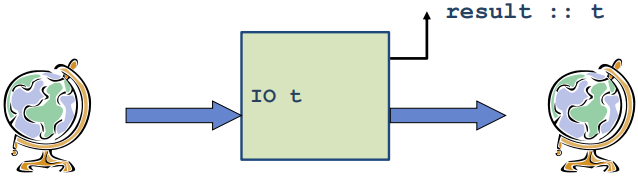
\includegraphics[width=300px]{images/7_Functional_Programming/IO_action.png}
\end{figure}
Moreover an action is a first-class value, evaluating an action has no effect while performing the action has the effect.
GHC uses the \emph{world-passing semantics} for the IO monad which represents the world by an un-forgeable token of type \verb|World| and implements bind and return as:
\begin{verbatim}
    return :: a -> IO a
    return a = \w -> (a, w)
    (>>=) :: IO a -> (a -> IO b) -> IO b
    (>>=) m k = \w -> case m w of (r, w') -> k r w'
\end{verbatim}
Using this form the compiler can do its normal optimizations, the dependence on the world ensures the resulting code will still be single-threaded.
The code generator then converts the code to modify the world in place.

\subsubsection{Simple I/O actions}
\begin{verbatim}
    getChar :: IO Char
    putChar :: Char -> IO ()

    main :: IO ()
    main = putChar 'x'
\end{verbatim}
So basically the main program is an action of type \verb|IO ()| and the basic operations are the \verb|getChar| to read a character and a \verb|putChar| to print a character.

\subsubsection{Bind combinator}
\begin{verbatim}
    (>>=) :: IO a -> (a -> IO b) -> IO b
\end{verbatim}
using the bind operator we can join two actions to make a new, bigger action:
\begin{verbatim}
    echo :: IO ()
    echo = getChar >>= putChar
\end{verbatim}

\subsubsection{Then combinator}
\begin{verbatim}
    (>>) :: IO a -> IO b -> IO b
\end{verbatim}
does sequencing when there is no value to pass.

\subsubsection{Return combinator}
\begin{verbatim}
    return :: a -> IO a
\end{verbatim}
the action \verb|return v| does no IO and immediately returns \verb|v|:

\subsubsection{do notation}
The do notation adds syntactic sugar to make monadic code easier to read, for example:
\begin{verbatim}
    getTwoChars :: IO (Char, Char)
    getTwoChars = getChar >>= \c1 ->
        getChar >>= \c2 ->
        return (c1, c2)
\end{verbatim}
can be rewritten in do notation using:
\begin{verbatim}
    getTwoCharsDo :: IO(Char, Char)
    getTwoCharsDo = do{
        c1 <- getChar;
        c2 <- getChar;
        return (c1 ,c2)
    }
\end{verbatim}
This syntax is designed to look imperative.

The scope of a variable bound in a generator is the rest of the do expression and we can have different syntaxes:
\begin{verbatim}
    do {x1 <- p1; ... ; xn <- pn; q}

    do x1 <- p1; ... ;  xn <- pn; q

    do x1 <- p1
        ...
        xn <- pn
        q
\end{verbatim}

\subsubsection{Some more examples}
We can join togheter some IO monadic operations in order to build bigger ones:
\begin{verbatim}
    getLine :: IO [Char]
    getLine = do {
        c <- getChar;
        if c == '\n then
            return []
        else do{
            cs <- getLine;
            return (c:cs)
        }
    }
\end{verbatim}

We can exploit monadic combinators to build control structures that work for any monadic type:
\begin{verbatim}
    repeatN :: (Num a, Monad m, Eq a) => a -> m a1 -> m ()

    repeatN 0 x = return ()
    repeatN n x = x >> repeatN (n-1) x

    for :: Monad m => [t] -> (t -> m a) -> m ()
    for []     fa = return ()
    for (x:xs) fa = fa x >> for xs fa
\end{verbatim}
we've built an implementation of the for loop which takes a function as parameter and is generic for every body which uses monadic operators:
\begin{verbatim}
    for [1..10] (\x -> putStr (show x))
\end{verbatim}

Moreover we can use the operators in order to give a sequencing to the actions:
\begin{verbatim}
    sequence :: Monad m => [m a] -> m [a]
    sequence [] = return []
    sequence (a:as) = do{
        r <- a;
        rs <- sequence as;
        return (r:rs)
    }
\end{verbatim}
this one too is generic for all the monadic operators and not only for the IO monad.

\subsubsection{Access to file}
IO monad has large collection of operations, a lot of them are similar to the C library functions for files:
\begin{verbatim}
    openFile :: FilePath -> IOMode -> IO Handle
    hPutStr  :: Handle -> String -> IO ()
    hGetLine :: Handle -> IO String
    hClose   :: Handle -> IO ()
\end{verbatim}

\subsubsection{References}
We can use IO operations to write more imperative things:
\begin{verbatim}
    data IORef a
    -- abstract type

    newIORef   :: a -> IO (IORef a)
    readIORef  :: IORef a -> IO a
    writeIORef :: IORef a -> a -> IO ()
\end{verbatim}
and a value of type \verb|IORef a| is a reference to a mutable cell holding a value of type \verb|a|.

\subsubsection{IO Monad as Abstract Data Type}
All operators of IO Monad returns an IO action, but only the bind operators takes one as argument, so bind is the only operation that combines IO actions, in order to force sequentiality.
So in Haskell there is no way to transform a value of type \verb|IO a| into a value of type \verb|a|, basically this means that in pure Haskell values from the external world can't become primitive types:
\begin{verbatim}
    configFileContents = lines (readFile "config")
    useOptimisation = "optimise" `elem` configFileContents
\end{verbatim}
this won't work because \verb|configFileContents| returns a list of \verb|IO String|, while \verb|"optimise"| is a \verb|String|.

To solve this problem we can:
\begin{itemize}
    \item write the entire program in IO monad, but this mean that we lose the simplicity of pure code;
    \item escape from the IO Monad using a function from \verb|IO String| to \verb|String|, but we can't... or we?
\end{itemize}

\subsubsection{Type-unsafe Haskell}
In case of IO action that doesn't matter when are actually executed Haskell offers another unsafe I/O primitive:
\begin{verbatim}
    unsafePerformIO :: IO a -> a
\end{verbatim}
The operator has a deliberately long name to discourage its use and its use comes with a \emph{proof obligation}, which means that we promise to the compiler that the timing of this operation relative to all other operations doesn't matter.




